\documentclass[b5paper,11pt,oneside,fleqn]{article}
\usepackage{amsmath,amsthm,amssymb}

\usepackage{graphicx}
\graphicspath{{gfx/}}
\usepackage{geometry}
\usepackage{xifthen}

\usepackage[svgnames, dvipsnames]{xcolor}
\definecolor{MyDarkGreen}{rgb}{0.0,0.4,0.0}
\definecolor{VlightBlue}{rgb}{.96,.98,1}
\definecolor{MyDarkBlue}{rgb}{.0,.0,0.3}
\definecolor{MyDarkRed}{rgb}{0.4, 0, 0}

\usepackage{listings}
\lstset{
        basicstyle=\small\ttfamily,             % Use small true type font
        columns=fullflexible,
        keepspaces=true,
        tabsize=2
}
% usage: \lstinputlisting[style=Matlab]{filename}

\lstdefinestyle{Matlab}{language=Matlab,        % Use MATLAB
%        frame=single,                          % Single frame around code
        basicstyle=\small\ttfamily,             % Use small true type font
        columns=fullflexible,
        keepspaces=true,
        keywordstyle=[1]\color{Blue}\bfseries,  %  MATLAB functions bold 
        %and blue
        keywordstyle=[2]\color{Purple},         %  MATLAB function arguments 
        %purple
        keywordstyle=[3]\color{Maroon}\bfseries,  % User functions 
        %underlined and blue
        identifierstyle=,                       % Nothing special about identifiers
                                                % Comments small dark green courier
        commentstyle=\usefont{T1}{pcr}{m}{tt}\color{MyDarkGreen},
%        commentstyle=\color{MyDarkGreen}\small,
        stringstyle=\color{Purple},             % Strings are purple
        showstringspaces=false,                 % Don't put marks in string spaces
        tabsize=2,                              % 5 spaces per tab
        %
        %%% Put standard MATLAB functions not included in the default
        %%% language here
        morekeywords={xlim,ylim,var,alpha,factorial,poissrnd,normpdf,normcdf,circshift,switch,
         case,otherwise,try,catch},
        %%%
        morekeywords={
AWG, 
callfemm, 
callfemm_noeval, 
ci_addarc, 
ci_addblocklabel, 
ci_addboundprop, 
ci_addconductorprop, 
ci_addmaterial, 
ci_addnode, 
ci_addpointprop, 
ci_addsegment, 
ci_analyse, 
ci_analyze, 
ci_attachdefault, 
ci_clearselected, 
ci_cleartkpoints, 
ci_close, 
ci_copyrotate, 
ci_copyrotate2, 
ci_copytranslate, 
ci_copytranslate2, 
ci_createmesh, 
ci_createradius, 
ci_deleteboundprop, 
ci_deleteconductor, 
ci_deletematerial, 
ci_deletepointprop, 
ci_deleteselected, 
ci_deleteselectedarcsegments, 
ci_deleteselectedlabels, 
ci_deleteselectednodes, 
ci_deleteselectedsegments, 
ci_detachdefault, 
ci_drawarc, 
ci_drawline, 
ci_drawpolygon, 
ci_drawpolyline, 
ci_drawrectangle, 
ci_getmaterial, 
ci_getview, 
ci_hidegrid, 
ci_hidenames, 
ci_loadsolution, 
ci_makeABC, 
ci_maximize, 
ci_minimize, 
ci_mirror, 
ci_mirror2, 
ci_modifyboundprop, 
ci_modifyconductorprop, 
ci_modifymaterial, 
ci_modifypointprop, 
ci_moverotate, 
ci_movetranslate, 
ci_movetranslate2, 
ci_probdef, 
ci_purgemesh, 
ci_readdxf, 
ci_refreshview, 
ci_resize, 
ci_restore, 
ci_saveas, 
ci_savebitmap, 
ci_savedxf, 
ci_savemetafile, 
ci_scale, 
ci_scale2, 
ci_selectarcsegment, 
ci_selectcircle, 
ci_selectgroup, 
ci_selectlabel, 
ci_selectnode, 
ci_selectrectangle, 
ci_selectsegment, 
ci_setarcsegmentprop, 
ci_setblockprop, 
ci_seteditmode, 
ci_setfocus, 
ci_setgrid, 
ci_setgroup, 
ci_setnodeprop, 
ci_setsegmentprop, 
ci_showgrid, 
ci_showmesh, 
ci_shownames, 
ci_snapgridoff, 
ci_snapgridon, 
ci_zoom, 
ci_zoomin, 
ci_zoomnatural, 
ci_zoomout, 
closefemm, 
complex2str, 
co_addcontour, 
co_bendcontour, 
co_blockintegral, 
co_clearblock, 
co_clearcontour, 
co_close, 
co_getconductorproperties, 
co_gete, 
co_getelement, 
co_getj, 
co_getk, 
co_getnode, 
co_getpointvalues, 
co_getprobleminfo, 
co_getv, 
co_getview, 
co_groupselectblock, 
co_hidecontourplot, 
co_hidedensityplot, 
co_hidegrid, 
co_hidemesh, 
co_hidenames, 
co_hidepoints, 
co_lineintegral, 
co_makeplot, 
co_maximize, 
co_minimize, 
co_numelements, 
co_numnodes, 
co_refreshview, 
co_reload, 
co_resize, 
co_restore, 
co_savebitmap, 
co_savemetafile, 
co_selectblock, 
co_selectpoint, 
co_seteditmode, 
co_setgrid, 
co_showcontourplot, 
co_showdensityplot, 
co_showgrid, 
co_showmesh, 
co_shownames, 
co_showpoints, 
co_showvectorplot, 
co_smooth, 
co_smoothoff, 
co_smoothon, 
co_snapgrid, 
co_snapgridoff, 
co_snapgridon, 
co_zoom, 
co_zoomin, 
co_zoomnatural, 
co_zoomout, 
create, 
ei_addarc, 
ei_addblocklabel, 
ei_addboundprop, 
ei_addconductorprop, 
ei_addmaterial, 
ei_addnode, 
ei_addpointprop, 
ei_addsegment, 
ei_analyse, 
ei_analyze, 
ei_attachdefault, 
ei_attachouterspace, 
ei_clearselected, 
ei_close, 
ei_copyrotate, 
ei_copyrotate2, 
ei_copytranslate, 
ei_copytranslate2, 
ei_createmesh, 
ei_createradius, 
ei_defineouterspace, 
ei_deleteboundprop, 
ei_deleteconductor, 
ei_deletematerial, 
ei_deletepointprop, 
ei_deleteselected, 
ei_deleteselectedarcsegments, 
ei_deleteselectedlabels, 
ei_deleteselectednodes, 
ei_deleteselectedsegments, 
ei_detachdefault, 
ei_detachouterspace, 
ei_drawarc, 
ei_drawline, 
ei_drawpolygon, 
ei_drawpolyline, 
ei_drawrectangle, 
ei_getmaterial, 
ei_hidegrid, 
ei_hidenames, 
ei_loadsolution, 
ei_makeABC, 
ei_maximize, 
ei_minimize, 
ei_mirror, 
ei_mirror2, 
ei_modifyboundprop, 
ei_modifyconductorprop, 
ei_modifymaterial, 
ei_modifypointprop, 
ei_moverotate, 
ei_movetranslate, 
ei_movetranslate2, 
ei_probdef, 
ei_purgemesh, 
ei_readdxf, 
ei_refreshview, 
ei_resize, 
ei_restore, 
ei_saveas, 
ei_savebitmap, 
ei_savedxf, 
ei_savemetafile, 
ei_scale, 
ei_scale2, 
ei_selectarcsegment, 
ei_selectcircle, 
ei_selectgroup, 
ei_selectlabel, 
ei_selectnode, 
ei_selectrectangle, 
ei_selectsegment, 
ei_setarcsegmentprop, 
ei_setblockprop, 
ei_seteditmode, 
ei_setfocus, 
ei_setgrid, 
ei_setgroup, 
ei_setnodeprop, 
ei_setsegmentprop, 
ei_showgrid, 
ei_showmesh, 
ei_shownames, 
ei_snapgridoff, 
ei_snapgridon, 
ei_zoom, 
ei_zoomin, 
ei_zoomnatural, 
ei_zoomout, 
eo_addcontour, 
eo_bendcontour, 
eo_blockintegral, 
eo_clearblock, 
eo_clearcontour, 
eo_close, 
eo_getconductorproperties, 
eo_getd, 
eo_gete, 
eo_getelement, 
eo_getenergydensity, 
eo_getnode, 
eo_getperm, 
eo_getpointvalues, 
eo_getprobleminfo, 
eo_getv, 
eo_groupselectblock, 
eo_hidecontourplot, 
eo_hidedensityplot, 
eo_hidegrid, 
eo_hidemesh, 
eo_hidenames, 
eo_hidepoints, 
eo_lineintegral, 
eo_makeplot, 
eo_maximize, 
eo_minimize, 
eo_numelements, 
eo_numnodes, 
eo_refreshview, 
eo_reload, 
eo_resize, 
eo_restore, 
eo_savebitmap, 
eo_savemetafile, 
eo_selectblock, 
eo_selectpoint, 
eo_seteditmode, 
eo_setgrid, 
eo_showcontourplot, 
eo_showdensityplot, 
eo_showgrid, 
eo_showmesh, 
eo_shownames, 
eo_showpoints, 
eo_showvectorplot, 
eo_smooth, 
eo_smoothoff, 
eo_smoothon, 
eo_snapgrid, 
eo_snapgridoff, 
eo_snapgridon, 
eo_zoom, 
eo_zoomin, 
eo_zoomnatural, 
eo_zoomout, 
hideconsole, 
hidepointprops, 
hi_addarc, 
hi_addblocklabel, 
hi_addboundprop, 
hi_addconductorprop, 
hi_addmaterial, 
hi_addnode, 
hi_addpointprop, 
hi_addsegment, 
hi_addtkpoint, 
hi_addtkpoints, 
hi_analyse, 
hi_analyze, 
hi_attachdefault, 
hi_attachouterspace, 
hi_clearselected, 
hi_cleartkpoints, 
hi_close, 
hi_copyrotate, 
hi_copyrotate2, 
hi_copytranslate, 
hi_copytranslate2, 
hi_createmesh, 
hi_createradius, 
hi_defineouterspace, 
hi_deleteboundprop, 
hi_deleteconductor, 
hi_deletematerial, 
hi_deletepointprop, 
hi_deleteselected, 
hi_deleteselectedarcsegments, 
hi_deleteselectedlabels, 
hi_deleteselectednodes, 
hi_deleteselectedsegments, 
hi_detachdefault, 
hi_detachouterspace, 
hi_drawarc, 
hi_drawline, 
hi_drawpolygon, 
hi_drawpolyline, 
hi_drawrectangle, 
hi_getmaterial, 
hi_getview, 
hi_hidegrid, 
hi_hidenames, 
hi_loadsolution, 
hi_makeABC, 
hi_maximize, 
hi_minimize, 
hi_mirror, 
hi_mirror2, 
hi_modifyboundprop, 
hi_modifyconductorprop, 
hi_modifymaterial, 
hi_modifypointprop, 
hi_moverotate, 
hi_movetranslate, 
hi_movetranslate2, 
hi_probdef, 
hi_purgemesh, 
hi_readdxf, 
hi_refreshview, 
hi_resize, 
hi_restore, 
hi_saveas, 
hi_savebitmap, 
hi_savedxf, 
hi_savemetafile, 
hi_scale, 
hi_scale2, 
hi_selectarcsegment, 
hi_selectcircle, 
hi_selectgroup, 
hi_selectlabel, 
hi_selectnode, 
hi_selectrectangle, 
hi_selectsegment, 
hi_setarcsegmentprop, 
hi_setblockprop, 
hi_seteditmode, 
hi_setfocus, 
hi_setgrid, 
hi_setgroup, 
hi_setnodeprop, 
hi_setsegmentprop, 
hi_showgrid, 
hi_showmesh, 
hi_shownames, 
hi_snapgridoff, 
hi_snapgridon, 
hi_zoom, 
hi_zoomin, 
hi_zoomnatural, 
hi_zoomout, 
ho_addcontour, 
ho_bendcontour, 
ho_blockintegral, 
ho_clearblock, 
ho_clearcontour, 
ho_close, 
ho_getconductorproperties, 
ho_getelement, 
ho_getf, 
ho_getg, 
ho_getk, 
ho_getnode, 
ho_getpointvalues, 
ho_getprobleminfo, 
ho_gett, 
ho_getview, 
ho_groupselectblock, 
ho_hidecontourplot, 
ho_hidedensityplot, 
ho_hidegrid, 
ho_hidemesh, 
ho_hidenames, 
ho_hidepoints, 
ho_lineintegral, 
ho_makeplot, 
ho_maximize, 
ho_minimize, 
ho_numelements, 
ho_numnodes, 
ho_refreshview, 
ho_reload, 
ho_resize, 
ho_restore, 
ho_savebitmap, 
ho_savemetafile, 
ho_selectblock, 
ho_selectpoint, 
ho_seteditmode, 
ho_setgrid, 
ho_showcontourplot, 
ho_showdensityplot, 
ho_showgrid, 
ho_showmesh, 
ho_shownames, 
ho_showpoints, 
ho_showvectorplot, 
ho_smooth, 
ho_smoothoff, 
ho_smoothon, 
ho_snapgrid, 
ho_snapgridoff, 
ho_snapgridon, 
ho_zoom, 
ho_zoomin, 
ho_zoomnatural, 
ho_zoomout, 
IEC, 
main_maximize, 
main_minimize, 
main_resize, 
main_restore, 
messagebox, 
mi_addarc, 
mi_addbhpoint, 
mi_addbhpoints, 
mi_addblocklabel, 
mi_addboundprop, 
mi_addcircprop, 
mi_addmaterial, 
mi_addnode, 
mi_addpointprop, 
mi_addsegment, 
mi_analyse, 
mi_analyze, 
mi_attachdefault, 
mi_attachouterspace, 
mi_clearbhpoints, 
mi_clearselected, 
mi_close, 
mi_copyrotate, 
mi_copyrotate2, 
mi_copytranslate, 
mi_copytranslate2, 
mi_createmesh, 
mi_createradius, 
mi_defineouterspace, 
mi_deleteboundprop, 
mi_deletecircuit, 
mi_deletematerial, 
mi_deletepointprop, 
mi_deleteselected, 
mi_deleteselectedarcsegments, 
mi_deleteselectedlabels, 
mi_deleteselectednodes, 
mi_deleteselectedsegments, 
mi_detachdefault, 
mi_detachouterspace, 
mi_drawarc, 
mi_drawline, 
mi_drawpolygon, 
mi_drawpolyline, 
mi_drawrectangle, 
mi_getmaterial, 
mi_hidegrid, 
mi_hidenames, 
mi_loadsolution, 
mi_makeABC, 
mi_maximize, 
mi_minimize, 
mi_mirror, 
mi_mirror2, 
mi_modifyboundprop, 
mi_modifycircprop, 
mi_modifymaterial, 
mi_modifypointprop, 
mi_moverotate, 
mi_movetranslate, 
mi_movetranslate2, 
mi_probdef, 
mi_purgemesh, 
mi_readdxf, 
mi_refreshview, 
mi_resize, 
mi_restore, 
mi_saveas, 
mi_savebitmap, 
mi_savedxf, 
mi_savemetafile, 
mi_scale, 
mi_scale2, 
mi_selectarcsegment, 
mi_selectcircle, 
mi_selectgroup, 
mi_selectlabel, 
mi_selectnode, 
mi_selectrectangle, 
mi_selectsegment, 
mi_setarcsegmentprop, 
mi_setblockprop, 
mi_setcurrent, 
mi_seteditmode, 
mi_setfocus, 
mi_setgrid, 
mi_setgroup, 
mi_setnodeprop, 
mi_setprevious, 
mi_setsegmentprop, 
mi_showgrid, 
mi_showmesh, 
mi_shownames, 
mi_snapgridoff, 
mi_snapgridon, 
mi_zoom, 
mi_zoomin, 
mi_zoomnatural, 
mi_zoomout, 
mo_addcontour, 
mo_bendcontour, 
mo_blockintegral, 
mo_clearblock, 
mo_clearcontour, 
mo_close, 
mo_geta, 
mo_getb, 
mo_getcircuitproperties, 
mo_getconductivity, 
mo_getelement, 
mo_getenergydensity, 
mo_getfill, 
mo_geth, 
mo_getj, 
mo_getmu, 
mo_getnode, 
mo_getpe, 
mo_getph, 
mo_getpointvalues, 
mo_getprobleminfo, 
mo_groupselectblock, 
mo_hidecontourplot, 
mo_hidedensityplot, 
mo_hidegrid, 
mo_hidemesh, 
mo_hidenames, 
mo_hidepoints, 
mo_lineintegral, 
mo_makeplot, 
mo_maximize, 
mo_minimize, 
mo_numelements, 
mo_numnodes, 
mo_refreshview, 
mo_reload, 
mo_resize, 
mo_restore, 
mo_savebitmap, 
mo_savemetafile, 
mo_selectblock, 
mo_selectpoint, 
mo_seteditmode, 
mo_setgrid, 
mo_showcontourplot, 
mo_showdensityplot, 
mo_showgrid, 
mo_showmesh, 
mo_shownames, 
mo_showpoints, 
mo_showvectorplot, 
mo_smooth, 
mo_smoothoff, 
mo_smoothon, 
mo_snapgrid, 
mo_snapgridoff, 
mo_snapgridon, 
mo_zoom, 
mo_zoomin, 
mo_zoomnatural, 
mo_zoomout, 
newdocument, 
num, 
numc, 
opendocument, 
openfemm, 
prompt, 
quote, 
quotec, 
rawquote, 
showconsole, 
showpointprops, 
smartmesh
        }
        %
        %%% Put MATLAB function parameters here
        morekeywords=[2]{on, off, interp},
        %
        %%% Put user defined functions here
        morekeywords=[3]{
calc_fluid_barrier,
draw_fluid_barrier
},
        %
        morecomment=[l][\color{Blue}]{...},     % Line continuation (...) like 
        %blue comment
        morecomment=[l]%
[\usefont{T1}{pcr}{m}{sl}%
\color{MyDarkGreen}%
\small\bfseries%
]{\%\%},     % Line 
        %continuation (...) like blue comment
%        numbers=left,                           % Line numbers on left
%        firstnumber=1,                          % Line numbers start with line 
%%1
%        numberstyle=\tiny,          % Line numbers are blue
%        stepnumber=2,                            % Line numbers go in steps of 
%%5
		backgroundcolor=\color{VlightBlue},
%        breaklines=true,
%        xleftmargin=7mm,
%        xrightmargin=0mm
    numbers=left,%none,%left,%
    numberstyle={\scriptsize\ttfamily\color{gray}},%\tiny
%    stepnumber=2,
%    numberfirstline=true,
%    numbersep=2pt,
    numbersep=1.5em,
%    firstnumber=auto,
    numberblanklines=false,
    tabsize = 2,
    showstringspaces=false,
    breaklines=true,
%    literate={\-}{}{0\discretionary{-}{}{}}, % delete -
    %frameround=ftff,
    %frame=single
    %  showlines=true,
    emptylines = 1,
    xleftmargin=1em,
    frame=l,
    framesep=2em,
    framexleftmargin=1em,%2.5mm,
    fillcolor=\color{VlightBlue!94!MyDarkBlue},
    framerule=2pt,
    rulecolor=\color{Maroon}
}

\makeatletter
\lst@CCPutMacro\lst@ProcessOther {"2D}{\lst@ttfamily{-{}}{-{}}}
\@empty\z@\@empty
\makeatother


\usepackage{tikz}
\usepackage{pgfplots}
\usetikzlibrary{calc,positioning,shapes.geometric,shapes.symbols,shapes.misc,arrows,math,arrows.meta}


\usepackage{filecontents}
\begin{filecontents}{fluid.bib}
@online{Bacco2018fluid,
title = {fluid: Free Fluid Flux-Barriers Rotor for Synchronous 
Reluctance Motor Drawing},
author = {Bacco, Giacomo},
journal = {GitHub},
url = {https://github.com/gbacco5/fluid},
urldate = {\today},
doi = {10.5281/zenodo.1214698},
date = {2018},
}
\end{filecontents}

\usepackage[
backend=biber,
style=alphabetic,
doi=true,
sorting=ynt
]{biblatex}
\addbibresource{fluid.bib}





\title{\raggedleft\sffamily\Huge fluid}
\author{\sffamily\itshape Bacco, Giacomo}
\date{}

\newcommand{\eu}{\mathrm{e}}
\newcommand{\je}{\mathrm{j}}

\newcommand{\ped}[1]{_\textup{#1}}
\newcommand{\ap}[1]{^\textup{#1}}
\newcommand{\pt}[1]{\mathsf{#1}}
\newcommand{\te}{\vartheta}
\newcommand{\Nstep}{N_{\textup{step}}}

% magnet width
\newcommand{\wm}[1][]{%
w_{\textup{m}
\ifthenelse{\isempty{#1}{}}{}{,#1}%
}}
% flux-carrier width
\newcommand{\wc}[1][]{%
w_{\textup{c}
\ifthenelse{\isempty{#1}{}}{}{,#1}%
}}
% flux-barrier thickness
\newcommand{\tb}[1][]{%
t_{\textup{b}
\ifthenelse{\isempty{#1}{}}{}{,#1}%
}}
% iron rib width
\newcommand{\wrib}[1][]{%
w_{\textup{rib}
\ifthenelse{\isempty{#1}{}}{}{,#1}%
}}
% tangential iron rib width
\newcommand{\wribt}{\wrib[\text{t}]}
\newcommand{\xth}[1]{$ #1 $-th}
% flux-barrier angle
\newcommand{\ab}[1][]{%
\alpha_{\textup{b}
\ifthenelse{\isempty{#1}{}}{}{,#1}%
}}

\newcommand{\pih}[1][]{\tfrac{\pi}{2#1}}
\newcommand{\map}{\mathcal{M}}
\newcommand{\de}{\partial}

\usepackage{url}
\usepackage{hyperref}

\newcommand{\nonfinito}{\emph{to be continued\ldots}}
\newcommand{\dirpath}{\texttt}

\begin{document}
\maketitle


\section*{Citing}
Please cite this work if you have used it in your project or in your program.
\vspace{0\baselineskip}

%{\small\noindent%
%Giacomo Bacco, \emph{fluid: Free Fluid Flux-Barriers Rotor for Synchronous 
%Reluctance Motor Drawing}, GitHub, 2018, available at:
%\url{https://github.com/gbacco5/fluid}
%}
{\noindent%
\fullcite{Bacco2018fluid}
}


\tableofcontents



\section*{Goal}
Provide a ready-to-use fully parametric drawing of the Synchronous Reluctance 
Rotor with fluid flux-barriers.

The scope of this project is the computation of the flux-barriers points.
The drawing scripts are for demonstration purposes only.


\section*{Requirements}
Matlab or Octave or Python (NumPy + SciPy) to compute the points.
The points calculation is general, so it could be implemented in any language, 
but I chose Matlab/Octave because it is my standard interface with 
\href{http://www.femm.info/}{FEMM} software.

If you do not use FEMM, you can still use the calculation part and make a 
porting for your CAD engine or FEA software. If you do so, consider 
contributing to the project adding your interface scripting.


\section{Files needed}

For Matlab/Octave, the files needed for the computation are

%\texttt{fluid.m} and 

\texttt{calc\_fluid\_barrier.m},

\texttt{GetFSolveOptions.m} and

\texttt{isOctave.m}


\noindent
while for Python it is

%\texttt{fluid.py} and 

\texttt{fluid\_functions.py}.



\newpage

\section*{Contacts}
You can contact me at
\href{mailto:giacomo.bacco@phd.unipd.it}{giacomo.bacco@phd.unipd.it}.

If you find a bug, consider opening an issue at 
\url{https://github.com/gbacco5/fluid/issues}

\vfill
{\footnotesize\noindent  Last update: \today}

\vspace{3cm}
Notice:
\lstinputlisting{../NOTICE.}



\clearpage
\section{How to use}

Open the file \lstinline|fluid| and run it.

Change the machine data in the data section.
All the variables have a comment next to them.

There are some ``hidden'' options which should be explained.
\begin{enumerate}
\item you can provide personal flux barrier angles, or let the program compute 
them as the average of the final points $ \pt{C} $ and $ \pt{D} $ at the rotor 
periphery.
This means that you have to always provide the flux-barrier thicknesses and 
flux-carrier widths.
Optionally, you could also provide the electrical flux-barrier angles.

\item by default, the flux-barrier-end is round, so the code solves an 
additional system to determine the correct locations of the fillet points.
You can skip such system declaring 
\begin{lstlisting}[style=Matlab]
rotor.barrier_end = 'rect';
\end{lstlisting}
and so selecting ``rectangular'' flux-barrier-end.

\item the inner radial iron ribs are optional, but you are free to provide 
different widths for every flux-barrier.
\begin{lstlisting}[style=Matlab]
rotor.wrib = [1,2,4]*mm;
\end{lstlisting}

\item if you also input magnet widths, the rib is automatically enlarged to 
accommodate the magnet, similarly to an IPM (Interior Permanent Magnet) machine.
\begin{lstlisting}[style=Matlab]
rotor.wm = [10,20,40]*mm;
\end{lstlisting}
In this case, the output structure \texttt{barrier} also contains the location 
of the magnet base center point.

\end{enumerate}



\clearpage
\section{Examples}
Here are some finished examples based on the output.
The drawings are for demonstration purposes only.

\vspace{\baselineskip}


\includegraphics[width=0.5\linewidth]{ex1}
\includegraphics[width=0.5\linewidth]{ex2}
\vspace{\baselineskip}

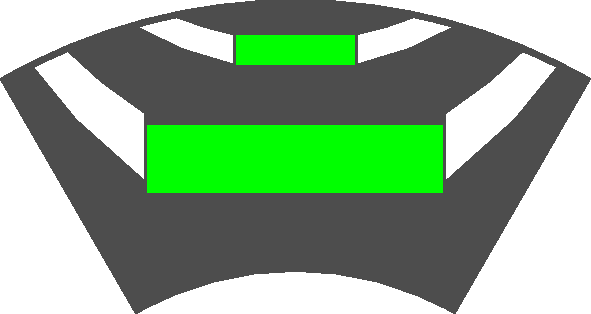
\includegraphics[width=0.75\linewidth]{ex3}




\clearpage
\section{Theory}

\subsection{Flow past a cylinder}

\begin{center}
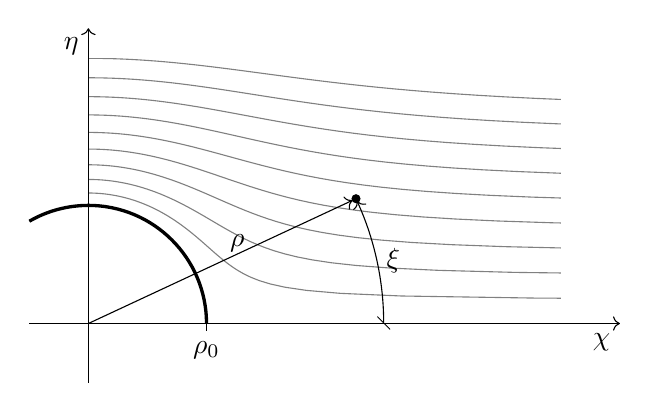
\begin{tikzpicture}
\def \Rzero {1.5cm};
\def \lvec {\Rzero/1.5};
%
% add streamlines
\begin{axis}[hide axis,
enlargelimits=false,
%xmin=0,xmax={6*\Rzero},
%ymin=0,ymax={3*\Rzero}
x = \Rzero, y=\Rzero,
%width={6*\Rzero}%,
%height={4*\Rzero},
ymin = 0,xmax=4%,
%axis background/.style={fill=white}
]
%
%\def \psidraw {0.1};
%
\foreach \psidraw in {0.2,0.4,...,1.8} {
\addplot [color=gray,domain=pi/128:pi/2,samples=50]
( {1*( (\psidraw + sqrt(\psidraw^2 + 4*(sin(deg(x)))^2 ))/(2*sin(deg(x))) 
)*cos(deg(x))} ,
{1*( (\psidraw + sqrt(\psidraw^2 + 4*(sin(deg(x)))^2 ))/(2*sin(deg(x))) 
)*sin(deg(x))} ) ; 
%(
%{ cos(deg(x)) },
%{ sin(deg(x)) }
%) ;
}
\end{axis}
%
% draw (x,y) reference frame
\draw [->] ({-\Rzero/2},0) -- ({4.5*\Rzero},0);
\node [anchor=north east] (abscissa) at ({4.5*\Rzero},0)
{$\chi$} ;
\draw [->] (0,{-\Rzero/2}) -- (0,{2.5*\Rzero});
\node [anchor=north east] (ordinate) at (0,{2.5*\Rzero})
{$\eta$} ;
%
\draw [very thick] (\Rzero,0cm) arc [start angle = 0, end angle = 120, 
radius=\Rzero];
\draw (\Rzero,1mm) -- (\Rzero,-1mm) node[anchor=north] {$\rho_0$};
% draw (rho,theta) ref. frame
\draw [->] (0,0) -- node[anchor=south west] {$ \rho $} (25:{2.5*\Rzero - 
0.5mm}) ;
\draw [fill=black] (25:{2.5*\Rzero}) circle [radius=0.5mm];
\draw [arrows = {|[slant=1]->}] (0:{2.5*\Rzero})
arc [start angle=0, end angle=24.5, radius={2.5*\Rzero}] 
node[midway,anchor=west]{$ \xi $};

%
%% add vectors of interest
%\coordinate (A) at ({5*\Rzero},\Rzero) ;
%\coordinate (B) at (75:\Rzero) ;
%\coordinate (C) at (0:{3.5*\Rzero}) ;
%\draw [-latex,NavyBlue,thick] (A) --
%node[anchor=south] {$ B_\infty $}
%node[anchor=north] {(\textsc{bc3})} ++(\lvec,0);
%\draw [-latex,Maroon,thick] (B) --
%node[anchor=east] {$ B_\rho = 0 $}
%node[anchor=west] {(\textsc{bc1})} ++(75:\lvec);
%\draw [-latex,OliveGreen,thick]
%(C) node[anchor=north] {$ B_\theta = 0 $} --
%++(90:\lvec) node[anchor=south] {(\textsc{bc2})};
%
\end{tikzpicture}
\end{center}



Let $ \rho_0 $ be the radius of the cylinder, $ \rho,\xi $ the polar coordinate
system in use.
One possible solution of this problem have these potential and streamline
functions:
\begin{align}
\phi(\rho,\xi) &= \left( \rho + \frac{\rho_0^2}{\rho} \right) \cos\xi 
\label{eq:potential}\\[1ex]
\psi(\rho,\xi) &= \left( \rho - \frac{\rho_0^2}{\rho} \right) \sin\xi
\label{eq:streamline}
\end{align}
Although these equations are deeply coupled, the radius $ \rho $ and the phase
$ \xi $ can be obtained as a function of the other quantities.
For our purposes, we use $ \psi $.
\begin{align}
\rho(\psi,\xi) &= \frac{\psi + \sqrt{\psi^2 + 4\rho_0^2 \sin^2\xi}}{2\sin\xi}
\\[1ex]
\xi(\psi,\rho) &= \arcsin \left( \frac{\rho\, \psi}{\rho^2 - \rho_0^2} \right)
\end{align}

The velocity field can also be derived through
\begin{equation}
\begin{aligned}
v_\rho(\rho,\xi)  &= \frac{\de\phi}{\de\rho} =
           \left( 1 - \frac{\rho_0^2}{\rho^2} \right) \cos\xi \\[1ex]
v_\xi(\rho,\xi)  &= \frac{1}{\rho} \frac{\de\phi}{\de\xi}  =
          -\left( 1 + \frac{\rho_0^2}{\rho^2} \right) \sin\xi
\end{aligned}
\end{equation}




\subsection{Conformal mapping}
From the reference plane, which is equivalent to a two-pole machine,
we use a complex map to obtain the quantities in the actual plane.
Let $ p $ be the number of pole pairs. Then:
\begin{equation}
\begin{aligned}
\zeta              &\xrightarrow{\;\map\;} z = \sqrt[p]{\zeta} \\
\rho\,\eu^{\je\xi} &\xrightarrow{\;\map\;}
                       r \, \eu^{\je\te} = \sqrt[p]{\rho}\,\eu^{\je
                       \xi/p} \\
\chi + \je\eta     &\xrightarrow{\;\map\;} x + \je y
\end{aligned}
\end{equation}
%
It is easy to find the inverse map:
\begin{equation}
\map\colon \sqrt[p]{\cdot} \qquad
\map^{-1}\colon (.)^p
\end{equation}

In the transformed plane, the velocities have a different expression:
\begin{equation}
\begin{aligned}
v_r(r,\te)  &=
p \left( r^{p-1} - \frac{R_0^{2p}}{r^{p+1}} \right) \cos p\te \\[1ex]
v_\te(r,\te)  &=
-p \left( r^{p-1} + \frac{R_0^{2p}}{r^{p+1}} \right) \sin p\te
\end{aligned}
\end{equation}
%
This vector field is tangent to the streamlines in every point in the
transformed plane. In order to work with this field in $ x,y $ coordinates, we
need a rotational map:
\begin{equation}
\begin{aligned}
v_x(r,\te) &= v_r \cos\te - v_\te \sin\te \\
v_\te(r,\te) &= v_r \sin\te + v_\te \cos\te
\end{aligned}
\end{equation}



\subsection{Computation of flux-barrier base points}

Refer to \autoref{fig: flux-barrier base points} for the points naming scheme.
Keep in mind that $ \pt{A}' $ is not simply the projection of $ \pt{A} $ onto 
the $ q $-axis, but it represent the original starting point for the barrier 
sideline, so it lies on the flux-barrier streamline. The same is true for 
points
$ \pt{B}',\pt{B} $, 
$ \pt{C}',\pt{C} $, and
$ \pt{D}',\pt{D} $.

\begin{figure}[tb]
\centering
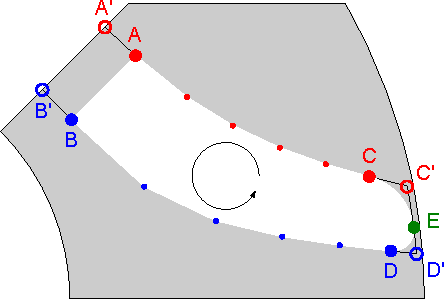
\includegraphics[width=0.75\linewidth]{gfx/BarrierPoints/BarrierPoints}
\caption{Flux-barrier base points description.}
\label{fig: flux-barrier base points}
\end{figure}

Let the flux-barrier and flux-carrier thicknesses be given.
Then the base points for the flux-barriers can be computed easily.
Let
$ D\ped{r} $ be the rotor outer diameter,
$ \wribt $ the tangential iron rib width,
$ \wc[k] $ the \xth{k} flux-carrier width,
and $ \tb[k] $ the \xth{k} flux-barrier thickness.%
\footnote{%
You may wonder why the main dimensions of the flux-carrier and
flux-barrier differ in the name (width versus thickness).
This is due to a choice of mine,
because I prefer to refer to width when the flux flows perpendicularly to the
dimension,
and to thickness when it flows in parallel.%
}
%
Then
\begin{equation}
\begin{aligned}
R\ped{r} &= \frac{D\ped{r}}{2} - \wribt \\
R_\pt{A_1'} &= R\ped{r} - \wc[1] \\
R_\pt{B_1'} &= R_\pt{A_1'} - \tb[1] \\
    &\:\:\,\vdots
\end{aligned}
\end{equation}
where $ R $ represents the radius from the origin.
%
So, in general:
\begin{equation}
\begin{aligned}
R_\pt{A_k'} &= R_\pt{B_{k-1}'} - \wc[k] \\
R_\pt{B_k'} &= R_\pt{A_{k-1}'} - \tb[k]
\end{aligned}
\end{equation}
with the exception $ R_\pt{B_0'} = R\ped{r} $.

Now we know both the radii and the angle -- always $ \pi/(2p) $ -- of the
flux-barrier internal points. So we can compute their respective streamline
value.



\subsubsection{Magnet insertion}
\[
\wrib[k] = \wrib[k] + \wm[k]
\]
where $ \wm[k] $ is the \xth{k} magnet width.


\subsubsection{Central base points}
We refer to points $ \pt{A} $ and $ \pt{B} $.
If the rib width is zero
$ \pt{A} \equiv \pt{A}' $ and
$ \pt{B} \equiv \pt{B}' $.

The line describing the $ q $-axis is
\begin{equation}
\begin{aligned}
y &= m x + q \\
m &= \tan\frac{\pi}{2p} \\
q &= \frac{\wrib}{2 \cos\frac{\pi}{2p}}
\end{aligned}
\end{equation}

\begin{equation}
\begin{cases}
y_\pt{A} - m x_\pt{A} - q = 0 \\
x_\pt{A} - r_\pt{A}(\psi_\pt{A'},\te_\pt{A}) \cos\te_\pt{A} = 0 \\
y_\pt{A} - r_\pt{A}(\psi_\pt{A'},\te_\pt{A}) \sin\te_\pt{A} = 0 \\
\end{cases}
\end{equation}
where $ \te_\pt{A} $ is used as the third degree of freedom and $ r_\pt{A} $ is
then a function of it.
The solution of such system can be determined solving the single equation
\begin{equation}
r_\pt{A}(\psi_\pt{A'},\te_\pt{A})
\bigl( \sin\te_\pt{A} - m \cos\te_\pt{A} \bigr) - q = 0
\end{equation}
in the unknown $ \te_\pt{A} $.
The function $ r(\psi,\te) $ is simply
\[
r(\psi,\te) = \sqrt[p]{ \rho(\psi,\te/p) \bigr) }
\]

The same equation can be written for point $ \pt{B} $ with the proper
substitution and repeated for all the flux-barriers.



\subsection{Outer base points}
We refer to points $ \pt{C} $, $ \pt{D} $, and $ \pt{E} $.
If the flux-barrier angle, $ \ab $, is given, then
\begin{equation}
\begin{aligned}
x_\pt{E} &= R_r \cos(\pih[p] - \ab) \\
y_\pt{E} &= R_r \sin(\pih[p] - \ab)
\end{aligned}
\end{equation}

Points $ \pt{C} $ and $ \pt{D} $ results from the connection of the
flux-barrier sidelines and point $ \pt{E} $.
This connection should be as smooth as possible in order to
avoid dangerous mechanical stress concentrations.
We are going to use circular arcs to make this connection.
So we impose the tangency between the flux-barrier sideline and the arc,
between the arc and the radius through point $ \pt{E} $.
The tangent to the sideline can be obtained through the velocity field
described above.

Then we want point $ \pt{C} $ to lay on the flux-barrier sideline. These
conditions represent a nonlinear system of 4 equations, in 6 unknowns.
So we need two more equations, which are that points $ \pt{C} $ and $ \pt{E} $
belong to the fillet circle with radius $ R $.
\begin{equation}
\begin{cases}
x_\pt{C} - r_\pt{C}(\psi_\pt{C}, \te_\pt{C}) \cos\te_\pt{C} = 0 \\
y_\pt{C} - r_\pt{C}(\psi_\pt{C}, \te_\pt{C}) \sin\te_\pt{C} = 0 \\
%
(x_\pt{C} - x_\pt{O_\pt{C}})^2 + (y_\pt{C} - y_\pt{O_\pt{C}})^2
- R_\pt{EC}^2 = 0 \\
(x_\pt{E} - x_\pt{O_\pt{C}})^2 + (y_\pt{E} - y_\pt{O_\pt{C}})^2
- R_\pt{EC}^2 = 0 \\
%
(x_\pt{O_\pt{C}} - x_\pt{E}) y_\pt{E} -
(y_\pt{O_\pt{C}} - y_\pt{E}) x_\pt{E} = 0 \\
%
(x_\pt{O} - x_\pt{C}) v_x(r_\pt{C},\te_\pt{C}) +
(y_\pt{O} - y_\pt{C}) v_y(r_\pt{C},\te_\pt{C})
\end{cases}
\end{equation}

The very same system can be written and solved for point $ \pt{D} $.



\subsection{Flux-barrier sideline points}

Consider the top flux-barrier sideline, so the one going from point $ \pt{A} $ 
to point $ \pt{C} $.
We want to create such sideline using a predetermined number of steps,
$ \Nstep $. From now on, let us call this number $ N $, 
and $ N_k $ for the $ k $-th flux-barrier.

One of the best way to distribute the points along the streamline is to use the 
potential function, $ \phi $, defined in \autoref{eq:potential}.
We start computing the potential for points $ \pt{A} $ and $ \pt{C} $:
\begin{equation*}
\begin{aligned}
\phi_\pt{A} &= \phi(\rho_\pt{A}, \xi_\pt{A}) \\
\phi_\pt{C} &= \phi(\rho_\pt{C}, \xi_\pt{C}) 
\end{aligned}
\end{equation*}
Then, we want to find $ N-1 $ points along the streamline
between points $ \pt{A} $ and $ \pt{C} $
with a uniform distribution of the potential function.
We define
\begin{equation*}
\Delta\phi_{\pt{AC}} = \frac{\phi_\pt{C} - \phi_\pt{A}}{N}
\end{equation*}
So we can compute the potentials we are looking for
\[
\phi_i = \phi_\pt{A} + i \Delta\phi_{\pt{AC}} \,,\quad i=1,\ldots,N-1
\]
and finally the location of the point with this potential value and the 
streamline function value required to lie on the flux-barrier sideline.
This translates to the following system of equations:
\begin{equation}
\begin{cases}
\psi_{\pt{AC}} - \psi(\rho,\xi) = 0 \\
\phi_i - \phi(\rho,\xi) = 0
\end{cases}
\end{equation}
The system is well-defined because there are two unknowns and two independent 
equations. This system must be solved for every flux-barrier sideline point, 
for the two sides, and for every flux-barrier.%
\footnote{In Matlab/Octave, the ``for every flux-barrier sideline point'' loop 
has been vectorized, while the two sides has been manually split.}


\subsection{Output}

The output of the computation function in Matlab/Octave is one vector of 
structures (\texttt{barrier(:)}) which contains at least two fields (\texttt{X} 
and \texttt{Y}).
%
The $ X $ vector is made in this way:
\[
X = 
\begin{bmatrix}
x_\pt{E} &
x_{\pt{O}_{\pt{C}}} & 
x_\pt{C} &
%
x_{\pt{AC}_{\Nstep-1}} &
\cdots &
x_{\pt{AC}_1} &
x_\pt{A} &
\searrow \\
%
x_\pt{B} & 
x_{\pt{BD}_1} &
\cdots &
x_{\pt{BD}_{\Nstep-1}} &
%
x_\pt{D} &
x_{\pt{O}_{\pt{D}}} & 
x_\pt{E} 
\end{bmatrix}\ap{T}
\]
and similarly the $ Y $ vector. So the points are ordered starting from the 
point $ \pt{E} $ and then moving counter-clockwise until $ \pt{E} $ is reached 
again.





\subsection{Example of Matlab/Octave plot}

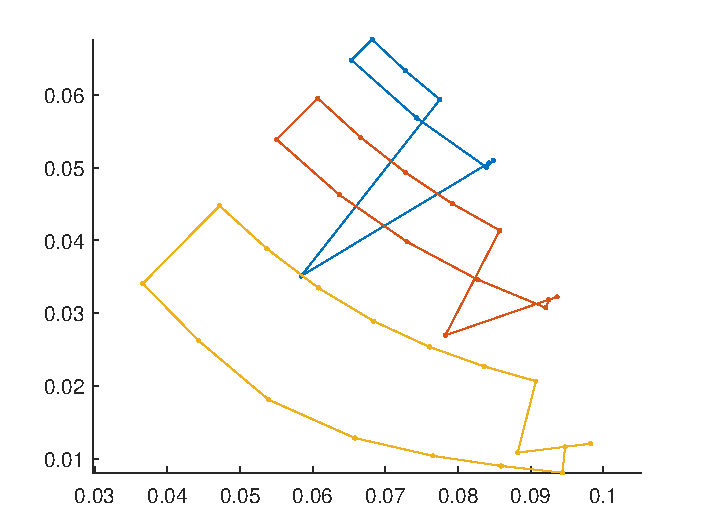
\includegraphics[width=0.75\linewidth]{gfx/MatlabOutput}

Here is an example of a Matlab/Octave output plot.
The V-shaped lines represent the radii of the fillet arcs, which were not worth 
to be shown in Matlab/Octave.




\clearpage
\section{Code}

\subsection{Main file}
\lstinputlisting[style=Matlab]{../fluid.m}
\clearpage

\subsection{Calc fluid barrier}
\lstinputlisting[style=Matlab]{../calc_fluid_barrier.m}
\clearpage

\subsection{Draw fluid barrier}
\lstinputlisting[style=Matlab]{../draw/draw_fluid_barrier.m}



\end{document}
